\section{Gantt-Diagramm}
Ein Gantt-Diagramm oder auch Balkenplan ist ein nach dem Unternehmensberater Henry L. Gantt benanntes Instrument des Projektmanagements, das die zeitliche Abfolge von Aktivitäten grafisch in Form von Balken auf einer Zeitachse darstellt.

In der Abbildung 1 sieht man die einzelnen Aktivitäten, die wir für unser Projekt Roboter-Fangen eingeplant haben.
Außerdem sieht

Einige Aktivitäten haben wir in Gruppen eingeteilt, um:
\begin{itemize}
	\item Planung
	\item Programmierung - Teil 1
	\item Programmierung - Teil 2
	\item Dokumentation
\end{itemize}

\begin{center}
	\begin{figure}[H]
		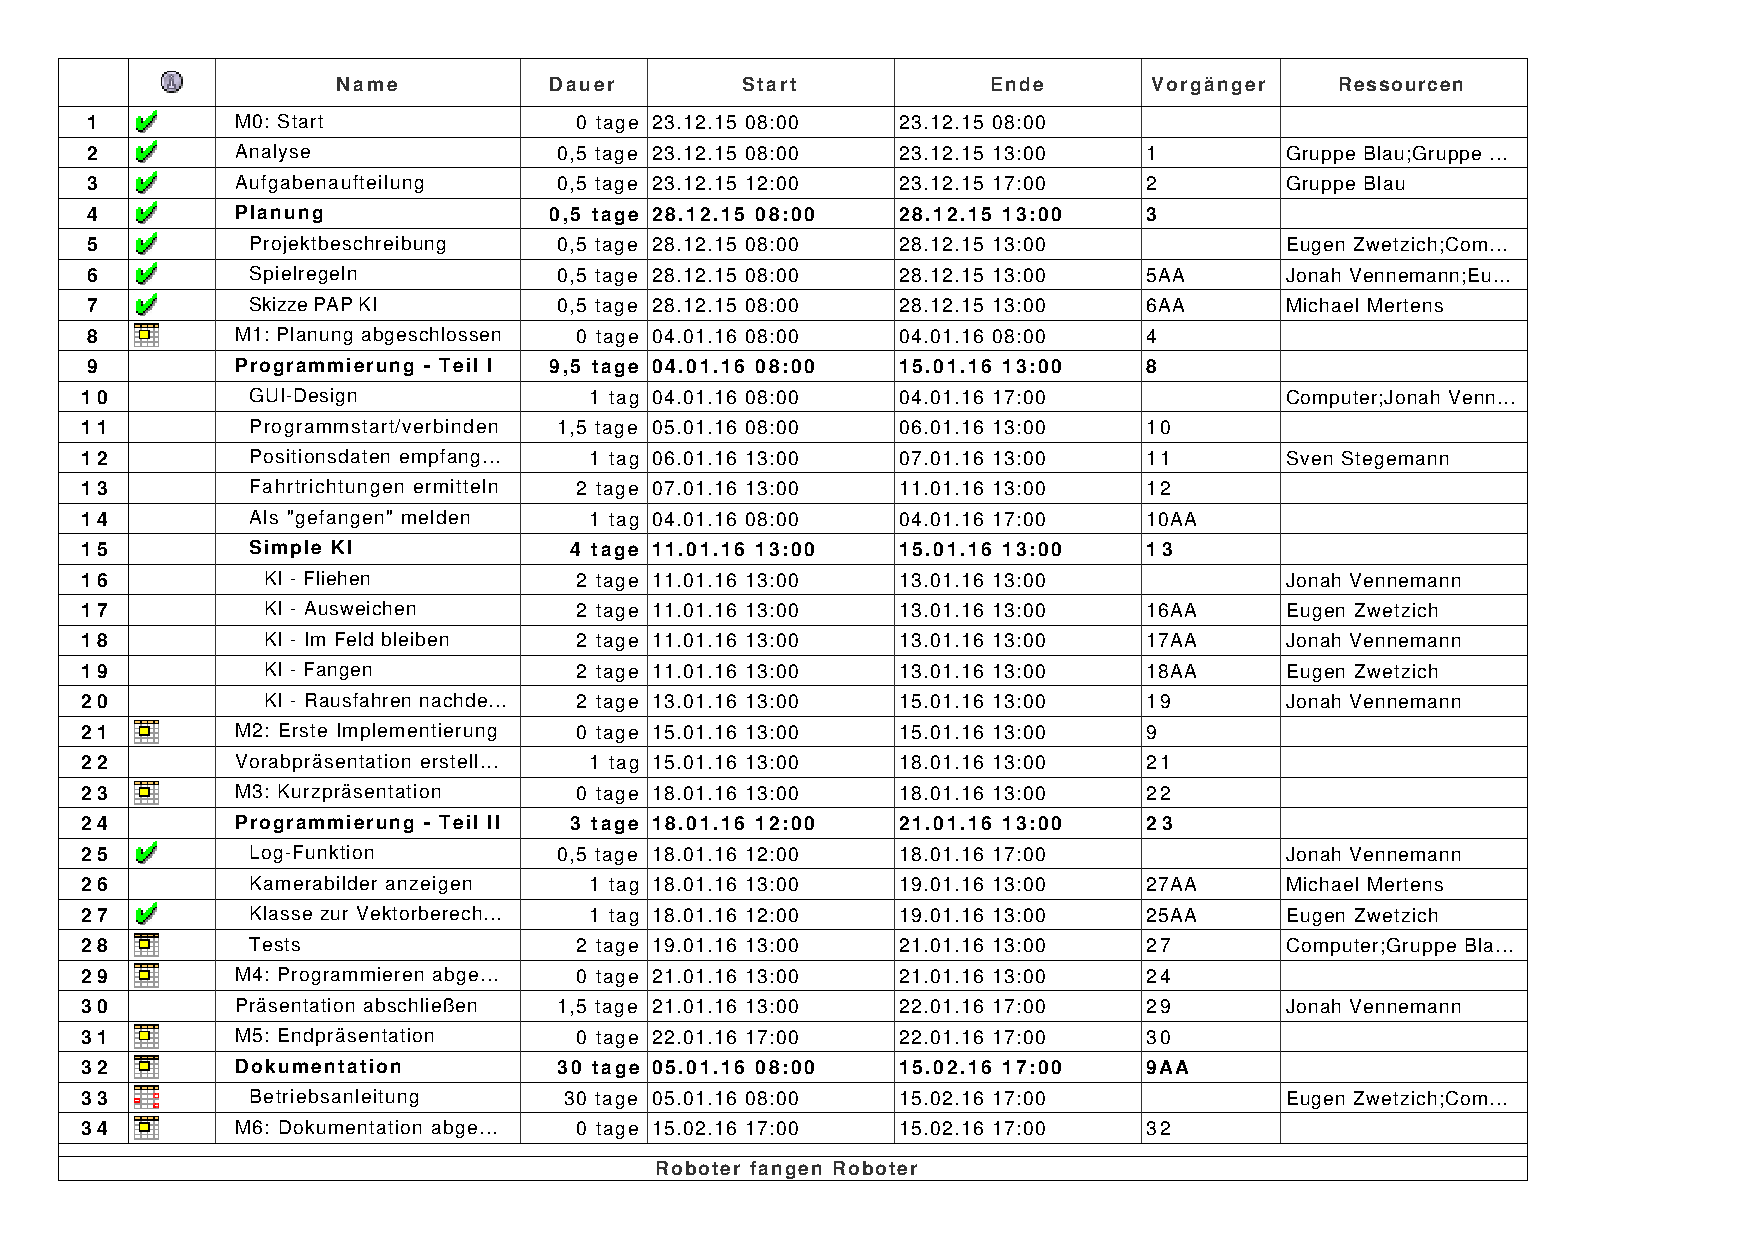
\includegraphics[scale=0.5]{Bilder/GanttDiagramm_[Page1].pdf}
		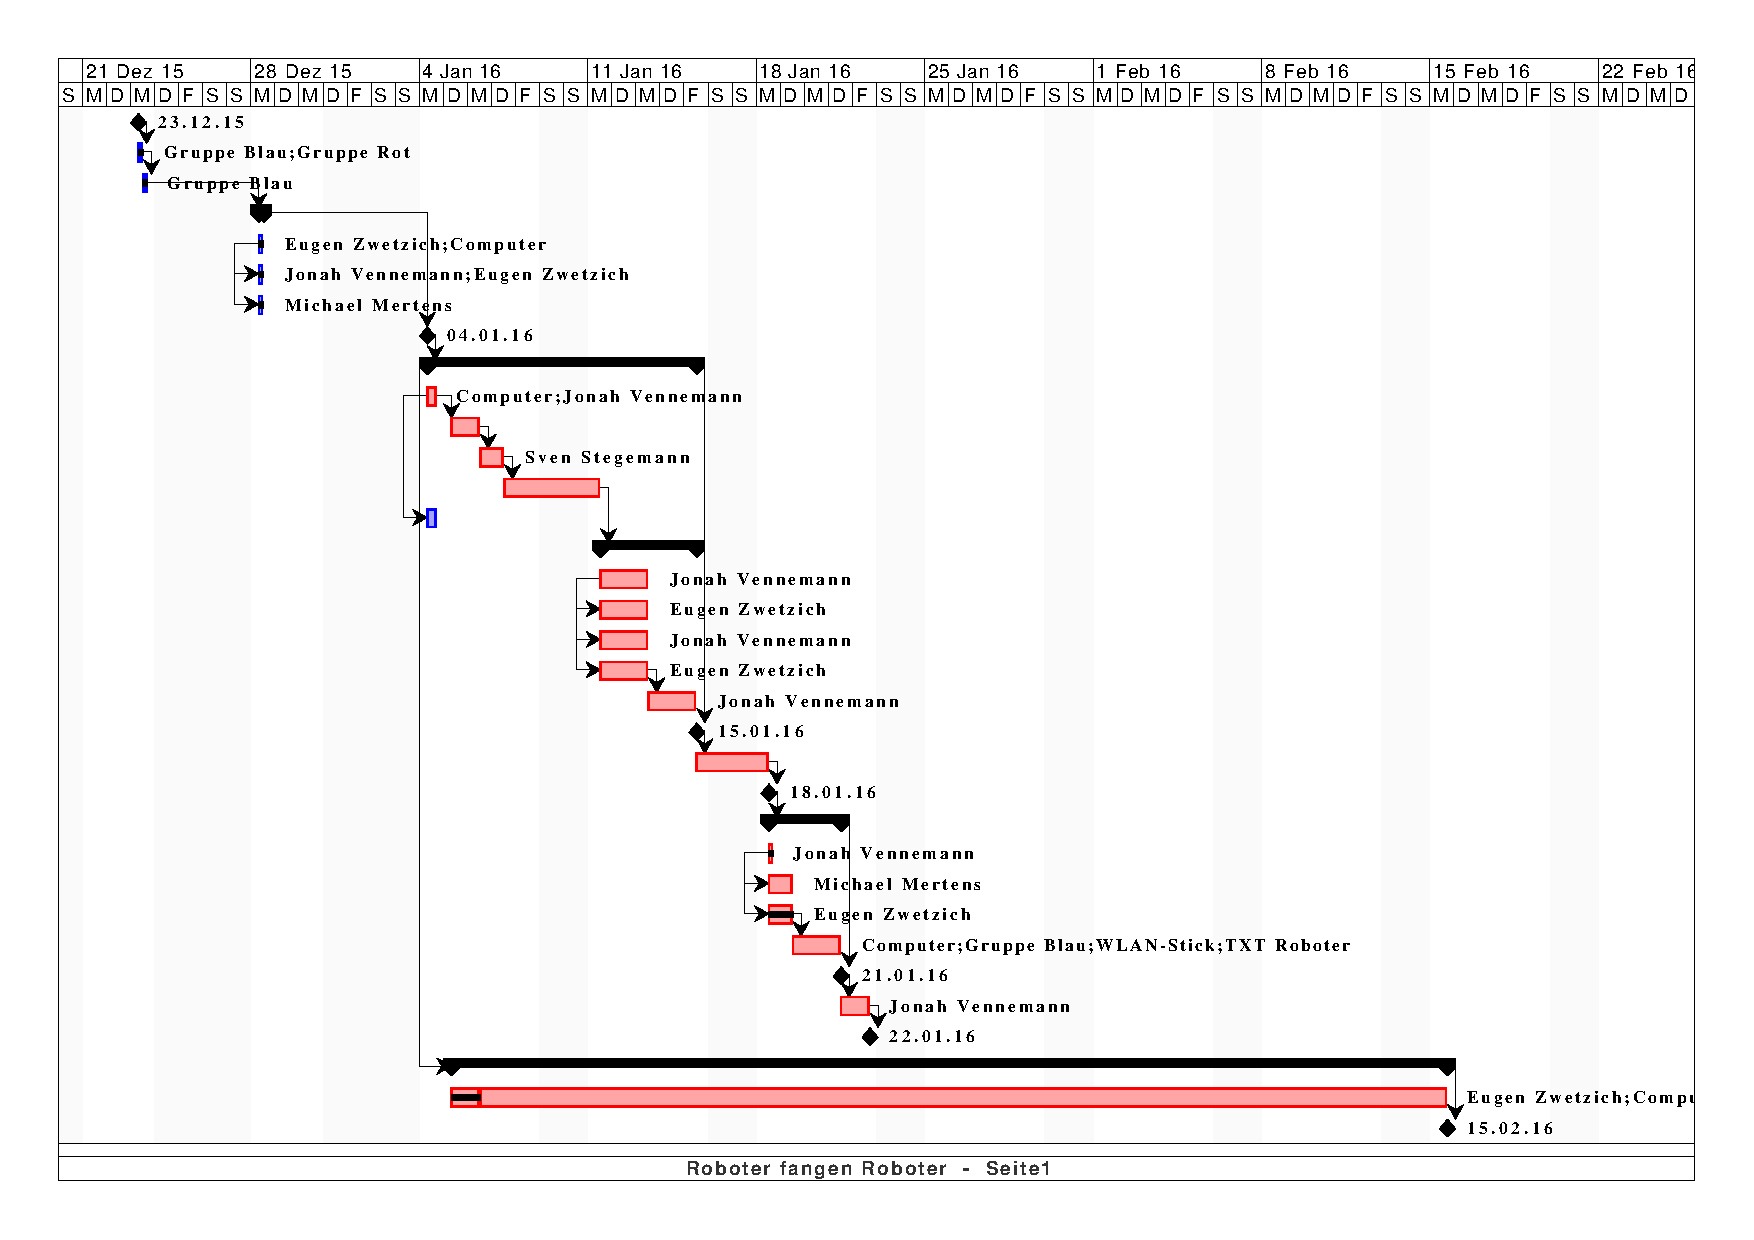
\includegraphics[scale=0.5]{Bilder/GanttDiagramm_[Page2].pdf}
		\caption{Gantt-Diagramm}
	\end{figure}
\end{center}
